\chapter*{The GECO Algorithm}
The main contribution of the authors in this paper is the GECO algorithm.\\
After explaining the "holes" and blurred reconstruction phenomena and enumerating the qualities of the $\beta$-VAE, the authors offer a principled approach to controlling the balance between the reconstruction error and the KL divergence.\\
Unlike $\beta$-VAE in which the machine learning practitioner must control the role of the unintuitive KL term, GECO optimizes the trade-off during training.
\subsection*{GECO Algorithm}
Initialize $t = 0$;\\
Initialize $\lambda = 1$;\\
\textbf{while} \textit{training} \textbf{do}:
\renewenvironment{description}[1][0pt]
  {\list{}{\labelwidth=0pt \leftmargin=#1
   \let\makelabel\descriptionlabel}}
  {\endlist}
\begin{description}[1cm]
\item Process current batch, x;
\item Sample from variational posterior $z\sim{q(z|x)}$
\item Compute empirical expectation of the reconstruction error $C^t = \mathcal{C}(x^t,g(z^t))$;
\item \textbf{if t is 0} then initialize the moving average of the reconstruction error, $C_{ma}^0 = C^0$
\item \textbf{else} $C_{ma}^t = \alpha C_{ma}^{t-1} + (1-\alpha)C^t$;
\item $C^t + StopGradient(C_{ma}^t - C^t)$
\item Update the parameters of the encoders and decoders using gradient descent
\item Update $\lambda$ using the update rule $\lambda^t = \lambda^{t-1}e^{\propto C^t}$
\item $t = t+1$
\end{description}

As stated earlier, the GECO algorithm optimizes the trade-off parameter that controls the relative importance of the KL term and the reconstruction error.\\
Additionally, by using e, $\lambda$ stays a positive number for all updates. This is a necessary requirement of optimization using the Lagrangian which is the mathematical basis of GECO. \\
The GECO algorithm allows the trade-off to change throughout training. For example, if the reconstruction error is higher then more weight may be given to the reconstruction error, thereby minimizing it.\\
This is important because often VAEs achieve the reconstruction error necessary for the human eye to not see any blurriness early on in training. However, after that point, when they are continually optimized, these VAEs minimize the reconstruction error at the expense of the KL term.\\
The authors show the significance of this in their empirical trials using ConvDraw trained on the CelebA and Color-MNIST data sets.\\
Below, we can see that using ELBO creates a latent space with blurriness and holes-results of the unnecessary reduction of the KL term in favor of the reconstruction error. In contrast, GECO achieves reconstruction that is visually equivalent with no holes or blurriness.\\

\begin{figure}[t]
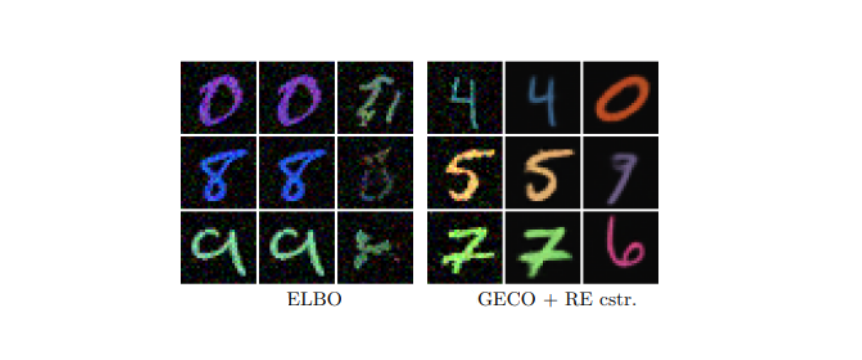
\includegraphics[width=\textwidth]{MNIST}
\caption{Note the differences in the last column of the ELBO dataset}
\centering
\end{figure}
\begin{figure}[t]
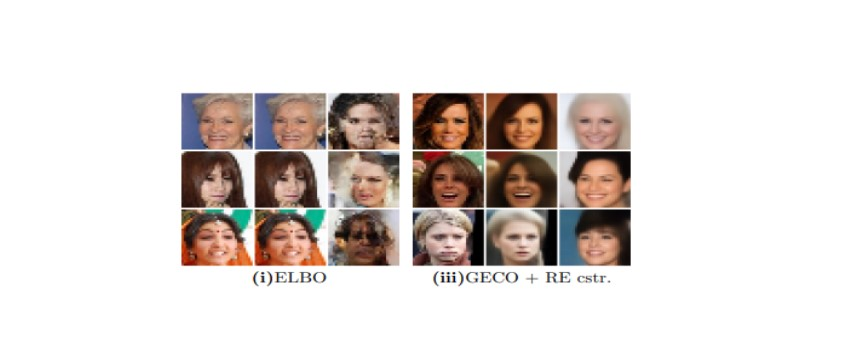
\includegraphics[width=\textwidth]{CelebA}
\caption{Note the differences in the last column of the ELBO dataset}
\centering
\end{figure}

	